\documentclass{standalone}
\usepackage{pgfplots}
\pgfplotsset{compat=1.18}

\begin{document}

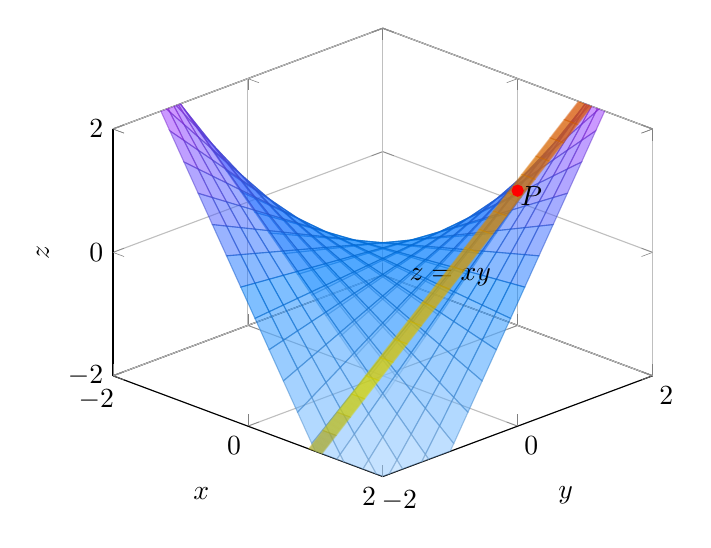
\begin{tikzpicture}
\begin{axis}[
    xlabel={$x$},
    ylabel={$y$},
    zlabel={$z$},
    xmin=-2, xmax=2,
    ymin=-2, ymax=2,
    zmin=-2, zmax=2,
    grid=major,
    view={45}{30}
]

% Surface z = xy with label
\addplot3[
    surf,
    opacity=0.5,
    colormap/cool,
    samples=20,
    domain=-2:2,
    domain y=-2:2,
]
{ x * y };
\node at (axis cs:1,0,0) {$z = xy$};

% Plane x = 1, parallel to yz-plane with a valid colormap
\addplot3[
    surf,
    opacity=0.3,
    colormap/hot, % Using a valid predefined colormap
    samples=20,
    domain=0.9:1.1,
    domain y=-2:2,
]
{ 1 * y };

% Mark the lattice point P (1,1,1) with label
\addplot3[only marks, mark=*, mark size=2pt, color=red] coordinates {(1,1,1)};
\node at (axis cs:1.2,1,1) {$P$};

\end{axis}
\end{tikzpicture}

\end{document}